\documentclass[10pt,a4paper]{ctexart}
\usepackage{amsmath,amssymb,bm}
\usepackage{graphicx}
\usepackage{booktabs,tabularx}
\usepackage[margin=1.2cm]{geometry}
\usepackage{hyperref}
\usepackage{caption}
\usepackage{enumitem}

\hypersetup{
  colorlinks=true,
  linkcolor=black,
  citecolor=black,
  urlcolor=black,
  pdftitle={MultiSpec-GeoDiff：多模态谱图驱动的几何分子结构反演},
}

\setlength{\parindent}{0pt}
\setlength{\parskip}{1.5pt plus 0.5pt}
\linespread{0.92}
\captionsetup{font=small,labelfont=small,skip=1pt}

\setlength{\abovedisplayskip}{3pt}
\setlength{\belowdisplayskip}{3pt}
\setlength{\abovedisplayshortskip}{2pt}
\setlength{\belowdisplayshortskip}{2pt}

\newcommand{\spec}{\mathcal S}
\newcommand{\R}{\mathbb R}

\begin{document}

\thispagestyle{empty}

{\LARGE\bfseries MultiSpec-GeoDiff：多模态谱图驱动的几何分子结构反演\par}
\vspace{3pt}
{\small\bfseries 谢翔宇\quad 中国科学技术大学\quad \href{mailto:xxy220348@mail.ustc.edu.cn}{xxy220348@mail.ustc.edu.cn}\par}
\vspace{4pt}
\hrule height 0.6pt
\vspace{4pt}

\section*{项目提议}

\textbf{具体目标：}拟构建多模态谱图驱动的几何分子结构反演模型，将反演形式化为几何约束下的多模态条件生成问题：
\[
\spec_{\mathrm{multi}} \rightarrow (c,C) \rightarrow G_{2D} \rightarrow D \rightarrow R^{(0)} \rightarrow (R,\mathcal T) \rightarrow \hat{\spec} \rightarrow \mathrm{TopK}.
\]

\textbf{核心价值：}谱图反演是一谱多解的逆问题——横坐标携带物理含义，分子具有图拓扑与三维几何。本方案以横坐标偏置注意力尊重物理坐标，以可增删节点图扩散自适应分子大小，以 pairwise distance 矩阵为 2D--3D 桥梁，以 TFN-Transformer 多阶张量特征与张量内积注意力实现 SE(3) 等变与手性建模，以前向谱图一致性验证候选，将反演从序列翻译提升至生成与验证闭环。

\textbf{可行性简析：}分三阶段推进——阶段一验证编码与候选重排闭环（已实现）；阶段二引入图扩散与距离预测；阶段三加入 parity-aware TFN-Transformer 与前向谱图闭环。数据来源包括 QM9S、NIST IR 及公开谱图数据库。风险为实验噪声与一谱多解。

\vspace{2pt}
{\centering
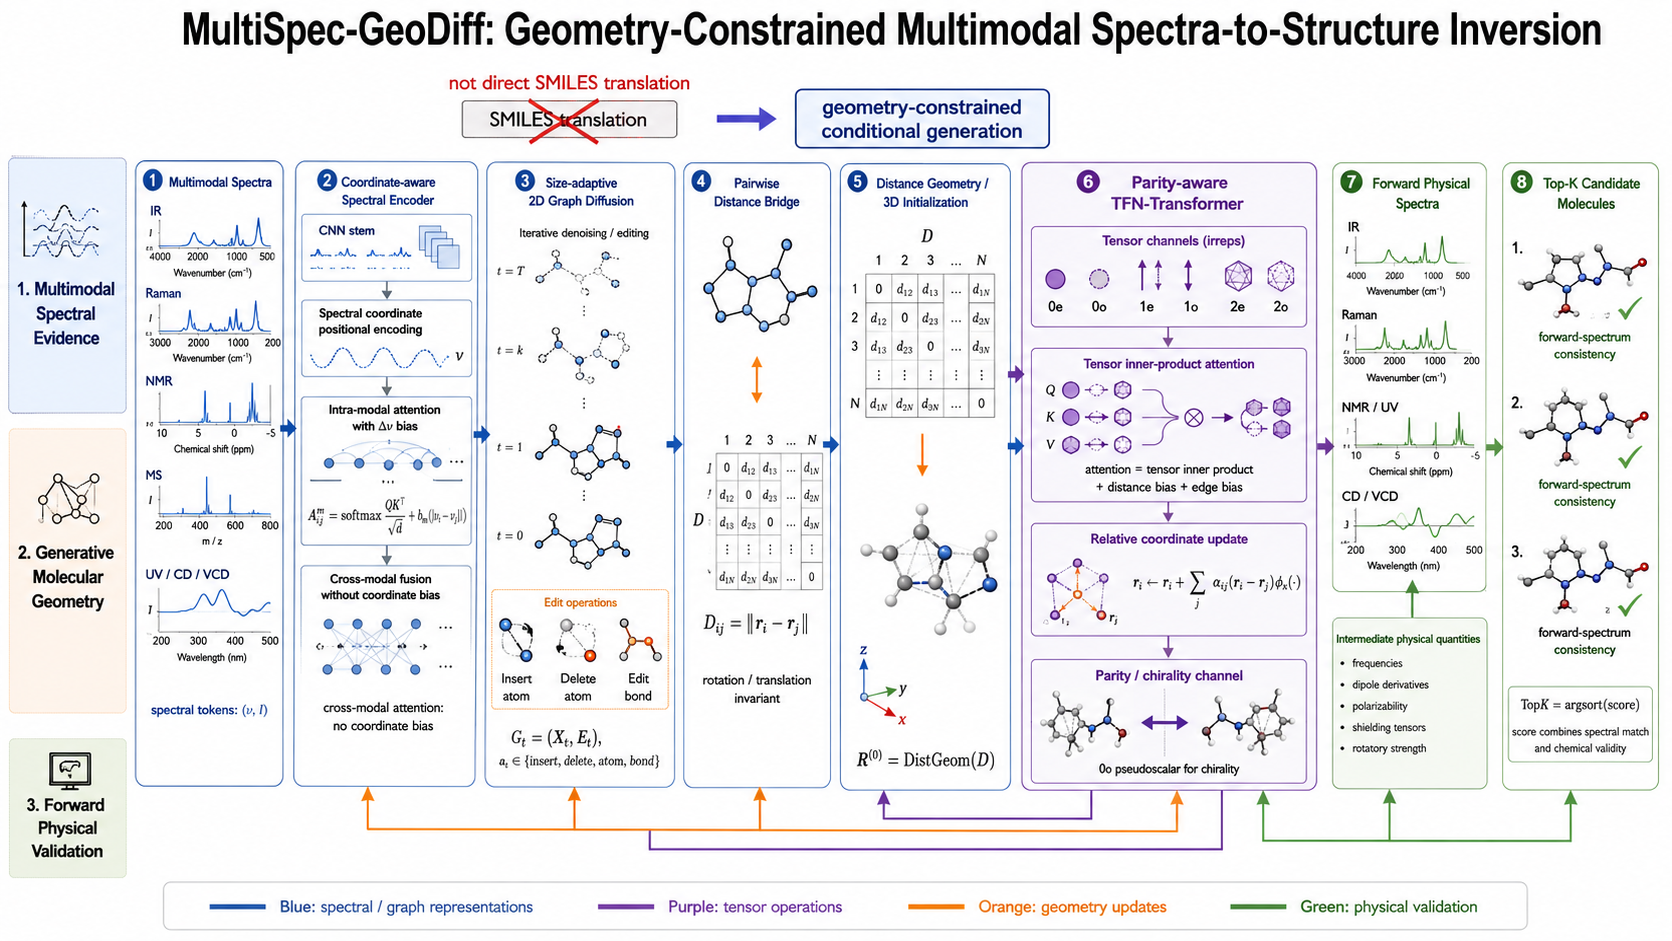
\includegraphics[width=\textwidth,height=0.42\textheight,keepaspectratio]{figures/fig0_overall_model_architecture.png}
\captionof{figure}{MultiSpec-GeoDiff 完整模型架构：多模态谱图经横坐标感知编码为条件表示，条件化二维图扩散、距离矩阵恢复、parity-aware TFN-Transformer 等变精修与前向谱图一致性重排。当前 MVP 已验证 IR/Raman 编码--候选召回--重排闭环；图扩散、距离预测与 TFN 精修为后续阶段。}\par}

\section*{核心数学结构}
\vspace{-3pt}

\textbf{1. 多模态谱图编码：从实验坐标到条件表示} \quad
谱图反演的输入不是无结构序列：每个点都携带物理横坐标与强度。多模态谱图表示为峰集合 $S^{(m)}=\{(\nu_i^{(m)},I_i^{(m)})\}_{i=1}^{L_m}$。CNN 提取局部峰形后，叠加模态编码与物理坐标位置编码：
\[
H_i^{(m,0)} = \mathrm{CNN}_m(I^{(m)})_i + e_m + p_m(\nu_i^{(m)}),\quad
p_m(\nu) = \mathrm{MLP}_m[\nu,\sin(\omega_1\nu),\cos(\omega_1\nu),\ldots].
\]
模态内自注意力引入真实横坐标距离偏置，使模型感知峰间物理间距：
\[
A_{ij}^{(m)} = \mathrm{softmax}_j\!\left(\frac{Q_i^{(m)}K_j^{(m)\top}}{\sqrt d} + b_m(|\nu_i^{(m)}-\nu_j^{(m)}|)\right).
\]
跨模态注意力不引入横坐标偏置（不同模态坐标系不可公度），仅学习证据兼容性：
\[
A_{ij}^{(m\leftarrow n)} = \mathrm{softmax}_j\!\left(\frac{Q_i^{(m)}K_j^{(n)\top}}{\sqrt d} + \gamma_{mn}\right).
\]
编码器输出全局条件 $c = \operatorname{Pool}(\{H^{(m)}\}_m)$ 与细粒度 token 条件 $C = \operatorname{Concat}(H^{(1)},\ldots,H^{(M)})$。得到 $(c,C)$ 后，谱图不再只是信号，而成为约束分子生成过程的条件场。

\textbf{2. 二维图扩散：从条件表示到候选分子图} \quad
谱图反演是一对多问题，生成比直接回归更自然；分子应先生成图为而非 SMILES。采用大小自适应图扩散，每一步允许原子增删与键变更：
\[
G_t = (X_t, E_t),\qquad a_t \in \{\mathrm{insert},\mathrm{delete},\mathrm{atom},\mathrm{bond}\},\qquad
D_\theta(G_t, t, c, C) \rightarrow a_t.
\]
反扩散 Graph Transformer 引入拓扑最短路径距离偏置与键类型偏置（Graphormer 风格）：
\[
\alpha_{ij} = \mathrm{softmax}_j\!\left(\frac{Q_iK_j^\top}{\sqrt d} + \beta_{\mathrm{SPD}(i,j)} + \eta_{e_{ij}}\right).
\]
输出 $G_{2D}=(X,E)$——二维图给出原子与化学键。但光谱响应还依赖三维几何；因此下一步不直接预测绝对坐标，而预测旋转平移不变的距离矩阵。

\textbf{3. Pairwise distance：2D 图到 3D 几何的桥梁} \quad
绝对坐标具有旋转平移规范歧义，而 pairwise 距离矩阵天然不变：$D_{ij}=\|r_i-r_j\|$、$D(R)=D(QR+t)$。先由 Graph Transformer 预测距离矩阵：
\[
\hat D = f_\theta(G_{2D}, c, C),\qquad \hat d_{ij} = \hat d_{ji} > 0,
\]
再经 Classical MDS 恢复初始坐标：
\[
B = -\tfrac12 J \hat D^{\circ 2} J,\ \ J = I - \tfrac1N \mathbf 1 \mathbf 1^\top,\qquad
B = U \Lambda U^\top,\ \ R^{(0)} = U_{:,1:3} \Lambda_{1:3}^{1/2}.
\]
可选损失 $\mathcal L_D = \sum_{i<j} |\hat D_{ij} - D_{ij}^{\mathrm{ref}}|^2$。距离几何只给出一个初始构象；真正的物理响应需要在三维空间中同时更新坐标与张量特征。

\textbf{4. TFN-Transformer：坐标、张量特征与等变注意力} \quad
各原子携带宇称分辨的多阶张量特征 $\mathcal T_i = \{T_i^{(l,p)}\}$（$l\in\{0,1,2\},\ p\in\{e,o\}$，即 $0e,0o,1e,1o,2e,2o$ 通道）。张量内积注意力权重为纯旋转不变量：
\[
s_{ij} = \sum_{l,p,c} \langle Q_{i,c}^{(l,p)}, K_{j,c}^{(l,p)}\rangle + b_{\mathrm{dist}}(\|r_i-r_j\|) + b_{\mathrm{edge}}(e_{ij}),\ \ \alpha_{ij} = \mathrm{softmax}_j(s_{ij}).
\]
TFN 消息传递通过球谐张量积实现等变特征交互：
\[
M_{ij}^{(l_3,p_3)} = \sum_{l_1,p_1,l_2,p_2} \phi(\|r_{ij}\|,e_{ij}) \bigl(T_j^{(l_1,p_1)} \otimes Y_{l_2}^{(p_2)}(\hat r_{ij})\bigr)_{l_3,p_3},\ \ p_3 = p_1p_2.
\]
坐标以 EGNN 风格相对更新：
\[
r_i^{(\ell+1)} = r_i^{(\ell)} + \sum_{j \neq i} \alpha_{ij} (r_i^{(\ell)}-r_j^{(\ell)})\, \phi_x(\|r_i-r_j\|^2, e_{ij}, \langle \mathcal T_i,\mathcal T_j\rangle_{\mathrm{tensor}}, c).
\]
输出 $(R,\mathcal T)=F_{\mathrm{TFN}}(G_{2D},R^{(0)},c,C)$。此时模型不再只是生成分子拓扑，而是在三维空间中形成可用于预测光谱响应的等变张量场。

\textbf{5. 手性与宇称：从几何对称性到 $0o$ 通道} \quad
手性不是普通标量信息。三重向量积 $\chi_{ijkl} = (r_j - r_i) \cdot [(r_k - r_i) \times (r_l - r_i)]$ 在旋转下不变、反射下反号，因此属于奇宇称标量（$0o$）通道：
\[
\chi \mapsto \chi\ (\mathrm{SO(3)}),\qquad \chi \mapsto -\chi\ (\mathrm{reflection}) \;\Longrightarrow\; \chi \in 0o.
\]
$0o$ 通道可在 CD/VCD/ROA 等手性敏感模态监督下编码手性信息。当前 MVP 尚未实现手性区分。

\textbf{6. 前向谱图一致性与 Top-K 后验重排} \quad
候选分子需经前向谱图验证。对每个 $(G_{2D,k}, R_k, \mathcal T_k)$：
\[
\hat{\spec}_k = F_{\mathrm{spec}}(G_{2D,k}, R_k, \mathcal T_k),\quad
s_k = -\operatorname{Dist}(\spec, \hat{\spec}_k) + \lambda_{\mathrm{chem}} S_{\mathrm{chem}}(G_k) + \lambda_{\mathrm{traj}} S_{\mathrm{diff}}(G_k).
\]
最终 $\operatorname{TopK} = \operatorname{argsort}_k(s_k)$。生成模块负责提出候选，前向谱图模块负责物理校验，二者共同形成谱图反演的闭环。后验重排可通过图神经网络（GNN）或等变 TFN 模块融合分子拓扑、三维几何与谱图特征实现。

\section*{阶段验证路线}
\vspace{-2pt}

\textbf{MVP（已完成）：}多模态 IR/Raman 横坐标感知编码、候选检索与 forward-spectrum reranking，输出 Top-K 及完整 trace。

\textbf{阶段二（近期）：}引入大小自适应图扩散生成分子图候选，pairwise distance 预测头联合训练。

\textbf{阶段三（远期）：}加入 parity-aware TFN-Transformer 等变精修与多阶张量谱图前向预测；扩展至 CD/VCD/ROA 等手性敏感模态。

\vspace{4pt}
\hrule height 0.4pt
\vspace{3pt}
{\small
受真实多模态实验谱图数据与量化标注成本限制，当前 demo 以轻量 toy 数据验证可执行闭环；其目标是证明技术路径可行性，而非报告生产级性能。完整研究计划需依赖更大规模公开/实验谱图数据库与量化弱监督。\\
项目仓库：\url{https://github.com/techandscixie2005/MultiSpec-GeoDiff-Demo}.}

\end{document}
